\documentclass[report]{nrel}

\usepackage[latin1]{inputenc}
\usepackage{amsmath}
\usepackage{amsfonts}
\usepackage{amssymb}
\usepackage{graphicx}
\usepackage{units}
\usepackage{moreverb}
\usepackage{siunitx}  %RRD
\sisetup{group-separator = {,}} %RRD
\DeclareSIUnit\year{yr}
\DeclareSIUnit\nmi{nmi}

\usepackage[
nonumberlist, %do not show page numbers
acronym,      %generate acronym listing
toc,          %show listings as entries in table of contents
section,      %use section level for toc entries
nomain]       %No main glossary 
{glossaries}

\usepackage{hyperref}
\urlstyle{rm} %RRD to put url in roman

\usepackage{array}          %RRD to help with table wrapping
\usepackage[flushleft]{threeparttable}       %RRD to help with tablenotes
\usepackage{tabularx,tabulary,longtable}       %RRD to help with table wrapping
\usepackage{multirow}       %RRD to help with table wrapping
\usepackage{textcomp} %RRD trademark
\usepackage{amsfonts}    %RRD to help with some math fonts

\renewcommand{\vec}[1]{\underline{#1}}

\graphicspath{../PICS/}     %RRD PICS folder path                             
%\usepackage[caption=false]{subfigure}


\newcommand\BibTeX{{\rmfamily B\kern-.05em \textsc{i\kern-.025em b}\kern-.08em
		T\kern-.1667em\lower.7ex\hbox{E}\kern-.125emX}}

%\usepackage[square]{natbib} %RRD
%\bibliographystyle{abbrvnat}
%\setcitestyle{authoryear, open={[(},close={)]}}


%Generate a list of symbols (acronyms are a default glossary)
%            log    name        in  out   title
\newglossary[syl]{symbolslist}{syi}{syo}{List of Symbols}
\newglossary[gkl]{greek}{kls}{klo}{Greek Symbols}

%Remove the dot at the end of glossary descriptions
\renewcommand*{\glspostdescription}{}

\let\firstchar\lowercase
\let\oldprintglossary\printglossary
\def\printglossary{\let\firstchar\uppercase\oldprintglossary}

% a bigger glossary description width:
\setlength\glsdescwidth{.9\textwidth}

%Activate glossary commands
\makeglossaries

%These commands sort the lists
%makeindex -s DynStall.ist -t DynStall.alg -o DynStall.acr DynStall.acn
%makeindex -s DynStall.ist -t DynStall.glg -o DynStall.gls DynStall.glo
%makeindex -s DynStall.ist -t DynStall.syl -o DynStall.syi DynStall.syo
\usepackage{glossary-mcols}
\setglossarystyle{mcolindex}


\def\ie{i.e., }
\def\eg{e.g., }
\def\cf{cf., }
\loadglsentries{glossary}

\makeglossaries
% \makenoidxglossaries

\def\ie{i.e.,}
\def\eg{e.g.,}
\def\cosa{\ensuremath{\cos{\alpha}}}
\def\sina{\ensuremath{\sin{\alpha}}}

\author{Rick Damiani}
\title{Theory Base for KiteFastMBD Preprocessor}

\addbibresource{C:/users/rdamiani/dropbox/references.bib}


\begin{document}
\glsdisablehyper

\frontmatter
\setcounter{page}{4}
\chapter*{Executive Summary}
This manual summarizes the theory and preliminary verifications of the \gls{ppc} module, which is part of \gls{kitefast} for airborne wind energy. 
The theory is largely based on the assumptions made in \gls{mbdyn} for its structural dynamics and beam element implementation. Specific assumptions made in \gls{kitefast}, as for example the straight axes for each component of the kite (\eg wings, stabilizers, fuselage), are also reflected in how the \gls{ppc} handles the stiffness distributions along the various beams.

  SOMETHING ABOUT THEORY AND VERIFICATION HERE. The results are encouraging, and future improvements to the code are recommended in this manual. 
%_______________________________________ %
\chapter*{Acknowledgments}
This work was supported by Makani Google X  under Contract No. with the National Renewable Energy Laboratory. 
%_______________________________________ %

\glsresetall


\tableofcontents

\listoffigures
\listoftables
\section*{\Large{List of Acronyms and Symbols}}\label{sec:symbols}
%\addcontentsline{toc}{section}{\nameref{sec:symbols}}%
\printglossary[type=\acronymtype,style=long]
\printglossary[type=symbols,style=long, title=Symbols]
\printglossary[type=greek,style=long, title=Greek Symbols]
\let\firstchar\lowercase %Reset to lowercase this command

\mainmatter
\lstset{language=[LaTeX]Tex,columns=fullflexible,keepspaces=true,breaklines=true}

%\maketitle


%\footnotetext[2]{Please ensure that you use the most up to date

%____________________________________________________________ %
\section{Overview}\label{sec:overview}
	
	The dynamics of semi-rigid kites can be simulated by combining  models for aerodynamics and structures. \gls{nrel} created a new software for the aeroelastic simulation of kites that makes use of \gls{mbdyn} as the core structural-dynamics solver and a series of modules that account for aerodynamics, tether dynamics, and control system. The software is called \gls{kitefast}. Multiple input files are necessary for the various parts of the software. To create \gls{mbdyn}'s input file, \gls{nrel} created a special \gls{ppc}. 
	
	This manual describes the main aspects of the theory developed and implemented in the \gls{ppc}. A detailed commentary of the input file needed for the \gls{ppc} is also given.
	
	The approximate way to distribute masses from cross-sectional properties at the first and third node of each element in a beam element is shown below. 
	
%__________________________________________________________________ %

\section{The 3-node Beam Elements and the Preprocessor}\label{sec:3node_beam}
The beam elements used in \gls{kitefast} are \gls{b3} or 3-node beam elements as described in \cite{masarati2017}. The preprocessor, starting from the end nodes (1 and 3) provided in the input file, will determine the middle node (node 2) location, and two intermediate (Gaussian) points. \gls{mbdyn} calculates internal forces and moments at the Gaussian points, which are located at $\gls{xihat}= \pm 1/\sqrt{3}$, where \gls{xihat} is the \glsentrydesc{xihat}. 

The stiffness matrices provided at the end nodes \emph{in the kite reference frame} are then transferred to the Gaussian point coordinates, based on a linear interpolation and the abscissa coordinate of the nodes and the Gaussian points.

The user is advised to guarantee sufficient resolution through the end node locations to capture any steep gradients along the various structural elements.

The beams are assumed straight, with reference (major) axis parallel to any one of the kite reference frame axes (x,y, or z). Each component node is therefore located along a constant pair of y,z or x,z or x,y coordinates. At each node, the user can define a twist angle about the beam reference axis that defines the orientation of the cross-section (\eg the airfoil pitch). 

\section{The Joints and the Preprocessor}\label{sec:joints}
Contiguous beam elements (for example along the starboard wing of the kite) are automatically joined at the common end-nodes. The subcomponents (wings, fuselage, pylons, stabilizers), however, need to be connected among each other unless they can share a physical structural node. For example, in the case of fuselage and either port or starboard wing, the connection can be realized via a `total joint' \citep{masarati2017}, which links the degrees of freedom of any two nodes belonging to the two components that must be connected.

In the case of a rotor and a pylon, the connection takes the form of a `revolute hinge' \citep{masarati2017}, which allows for a relative rotation along the z-axis of a reference frame common to the two nodes to be connected.
 
The \gls{ppc} sets up all the necessary connections based on the definitions of the various subcomponents,  the 'attached component' syntax, and the component keypoint definition (see also Section~\ref{sec:inputfile}). 

Note that the attached components are specified following the hierarchy with which they were defined; for example, to specify that the lower port rotor is connected to a pylon node, the syntax in the input file is "rotor\_assembly/lower/port/2" or "rotor\_assembly/port/lower/2" where the order does not need to be fixed (see Section~\ref{sec:inputfile}). 

%___________________________________________________________________________________________ %
\section{Mass Distribution Theory}\label{sec:massdist}
The \gls{b3} requires three concentrated masses and inertia at the three nodes. There is no general way to specify masses at the nodes, and the hope is to reduce the error by matching at the end the overall integral (\gls{3d}) inertial properties of the beam element. 

In this treatment, we assume that the beam element is rectilinear. For curved beams the theory should be revised.

The main assumption is that the mass and the inertias are modeled as linear distributions.
For simplicity's sake, we assume that the coordinate system has the origin at \gls{n1}, with the x-axis along the beam element, consistent with \gls{mbdyn}.

The beam's mass (\gls{Mass}) and center of mass coordinates (\gls{Xg},\gls{Yg},\gls{Zg}) can be calculated as:
%
\begin{align}\label{eq:beamCg}
	\gls{Mass}  = \int_{0}^{\gls{lb}}\gls{mx} dx \\
	\gls{Xg}    = \dfrac{\int_{0}^{\gls{lb}}\gls{mx} \gls{xg} dx}{\gls{Mass}} \\
	\gls{Yg}    = \dfrac{\int_{0}^{\gls{lb}}\gls{mx} \gls{yg} dx}{\gls{Mass}} \\
	\gls{Zg}    = \dfrac{\int_{0}^{\gls{lb}}\gls{mx} \gls{zg} dx}{\gls{Mass}} 
\end{align}
%
where \gls{lb} is the \glsentrydesc{lb}; \gls{mx} is the \glsentrydesc{mx}; \gls{xg}--\gls{zg} are the coordinates as a function of x of the cross-sectional center of mass. 

Analogously, we can write the inertial quantities:
%
\begin{align}\label{eq:beamI}
	\gls{Ixx}  = \int_{0}^{\gls{lb}} \left[ \gls{ixx} + \gls{mx}\left(\gls{yg}^2+\gls{zg}^2 \right)      \right] dx \\
	\gls{Iyy}  = \int_{0}^{\gls{lb}} \left[\gls{iyy} + \gls{mx}\left(\gls{xg}^2+\gls{zg}^2 \right)      \right] dx \\
	\gls{Izz}  = \int_{0}^{\gls{lb}} \left[\gls{izz} + \gls{mx}\left(\gls{xg}^2+\gls{yg}^2 \right)      \right] dx \\
	\gls{Ixy}  = \int_{0}^{\gls{lb}} \left[ \gls{ixy} + \gls{mx} \left( \gls{xg}\gls{yg} \right)      \right] dx \\
	\gls{Ixz}  = \int_{0}^{\gls{lb}} \left[ \gls{ixz} + \gls{mx} \left( \gls{xg}\gls{zg} \right)      \right] dx \\
	\gls{Iyz}  = \int_{0}^{\gls{lb}} \left[ \gls{iyz} + \gls{mx} \left( \gls{yg}\gls{zg} \right)      \right] dx 
\end{align}
%
where \gls{ixx}--\gls{izz} are the cross-sectional second moments of inertia about the centroidal axes as a function of the beam's span x.

Note that because the beam axis is considered along x, $\gls{xg}=x$. 

The inputs are the quantities \gls{mx}, \gls{xg}--\gls{zg}, and \gls{ixx}--\gls{izz} at the end nodes (1st and 3rd node) of the beam. By assuming linear functions of $x$ for all of these quantities, all of the above integral quantities can be analytically calculated. The expressions of the typical terms are given in Eq.~\eqref{eq:integrals}:
%
\begin{equation}\label{eq:integrals}
	\renewcommand*{\arraystretch}{2.5}
	\begin{array}{ll}
	    \gls{mx}   =  a x + b \\
	  	\gls{ixx} (\textrm{or} \quad \gls{iyy}, \gls{ixy}, ...)  = c x + d \\
	  	\gls{yg}   =  e x + f  \\
	  	\gls{zg}   =  g x + h  \\
	  	\gls{mx}\gls{yg} = ae x^2 + (af+be)x +bf \\
	  	\gls{yg}\gls{zg}  =  eg  x^2  + (eh+fg)x + fh \\
	  	\gls{mx}\gls{yg}\gls{zg}  =  aeg  x^3  + \left( a(eh+fg) + beg \right)x^2 + \left( afh +b(eh+fg) \right) x + bfh \\
	  	\gls{yg}^2 + \gls{zg}^2  =  (e^2+g^2) x^2  + 2(ef+gh)x + (f^2+h^2) \\
%
	  	\gls{mx}\left(\gls{yg}^2 + \gls{zg}^2\right) = a(e^2+g^2) x^3 + \left(2a(ef+gh) + b(e^2+g^2) \right)x^2 + \left( a (f^2+h^2) + 2b(ef+gh) \right) x  +b(f^2+h^2) \\
%
		\gls{Mass} = a \dfrac{\gls{lb}^2}{2} + b\gls{lb} \\
%
		\gls{Yg}   = ae \dfrac{\gls{lb}^3}{3} + (af+be)\dfrac{\gls{lb}^2}{2} + bf \gls{lb} \\
%
		\gls{Ixx}  =\int_{0}^{\gls{lb}} \left[ \gls{ixx} + \gls{mx}\left(\gls{yg}^2+\gls{zg}^2 \right)      \right] dx = \\
			\quad \left[ a(e^2+g^2) \dfrac{\gls{lb}^4}{4}  +
			 \left(2a(ef+gh) + b(e^2+g^2) \right)\dfrac{\gls{lb}^3}{3} + 
			 \left( a (f^2+h^2) + 2b(ef+gh) + c \right) \dfrac{\gls{lb}^2}{2}+
			 \left( b(f^2+h^2) + d \right) \gls{lb} \right] \\
%
		\gls{Iyy}  = \int_{0}^{\gls{lb}} \left[c x + d + \gls{mx}\left(x^2+\gls{zg}^2 \right)      \right] dx =\\	
			\quad	\left[ a(1+g^2) \dfrac{\gls{lb}^4}{4}  +
			\left(2a(gh) + b(1+g^2) \right)\dfrac{\gls{lb}^3}{3} + 
			\left( a (h^2) + 2b(gh) + c \right) \dfrac{\gls{lb}^2}{2}+
			\left( b h^2 + d \right) \gls{lb} \right] \\
%
		\gls{Ixy}  = \int_{0}^{\gls{lb}} \left[ \gls{ixy} + \gls{mx} \left( \gls{xg}\gls{yg} \right)      \right] dx = 	\int_{0}^{\gls{lb}} \left[ c x + d + \gls{mx} \left( x\gls{yg} \right)      \right] dx =\\			
			\quad	\int_{0}^{\gls{lb}} \left[ae  x^3  + \left( af + be \right)x^2 + \left(  bf + c\right) x  +d \right] dx= ae  \dfrac{\gls{lb}^4}{4}  + \left( af + be \right)\dfrac{\gls{lb}^3}{3} + \left(  bf + c\right) \dfrac{\gls{lb}^2}{2}  +d \gls{lb} \\
%			
		\gls{Iyz}  = \int_{0}^{\gls{lb}} \left[ \gls{iyz} + \gls{mx} \left( \gls{yg}\gls{zg} \right)      \right] dx = \int_{0}^{\gls{lb}} \left[ aeg  x^3  + \left( a(eh+fg) + beg \right)x^2 + \left( afh +b(eh+fg) +c\right) x + (bfh +d)      \right] dx =\\
			\quad	aeg  \dfrac{\gls{lb}^4}{4}  + \left( a(eh+fg) + beg \right) \dfrac{\gls{lb}^3}{3} + \left(  afh +b(eh+fg) +c \right) \dfrac{\gls{lb}^2}{2}  +(bfh +d) \gls{lb} \\
	
	\end{array}
\end{equation}
%
where the constants $a,b,c,d,e,f,g,h$ are calculated for each of the parameters from the values at the two nodes as for example:
\begin{equation}\label{eq:linearConst}
	\renewcommand*{\arraystretch}{2.5}
	\begin{array}{lcl}
		d &=& \gls{ixx1} \\
		c &=& \dfrac{\gls{ixx3}-\gls{ixx1}}{\gls{lb}}
		\end{array}
\end{equation}
%
where \gls{ixx1} and \gls{ixx3} are the beam's cross-sectional second mass moments of inertia about the centroidal x-axis at first and last node of the beam element, respectively.

The goal is to find three nodal masses and associated inertia tensors that can as-close-as-possible match the same integral quantities.
This translates into 27 unknowns: \gls{Mi}, \gls{Ygi}, \gls{Zgi}, \gls{Ixxi},  \gls{Iyyi},  \gls{Izzi}, \gls{Ixyi},  \gls{Ixzi},  and \gls{Iyzi} with $i=1..3$, where: \gls{Mi} is the \glsentrydesc{Mi}; \gls{yi}, \gls{zi} are the \glsentrydesc{yi} and \glsentrydesc{zi}, respectively; \gls{Ixxi}--\gls{Izzi} and \gls{Ixyi}--\gls{Iyzi} are the second moments of inertias and the skew moments of inertias associated with the nodal lumped masses.
%
\begin{figure}[h]
	\centering
	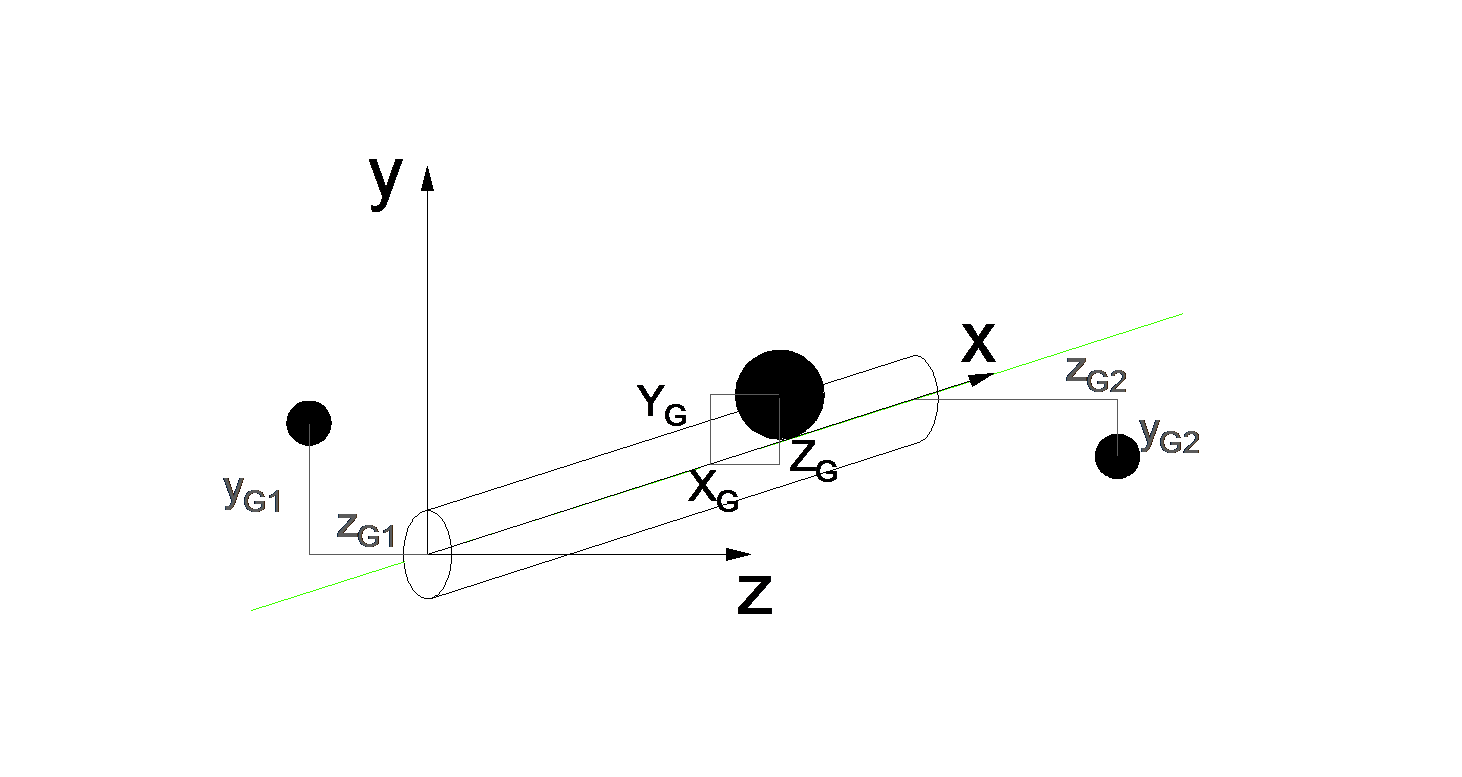
\includegraphics[width=0.8\linewidth]{PICS/beam2}
	\caption{Diagram showing one 2-node subelement and the lumped masses at the nodes and the overall mass lumped at the center of mass of the beam element.}
	\label{fig:beam2}
\end{figure}
%

It is convenient to subdivide the 3-node beam element into two 2-node elements (see Fig.~\ref{fig:beam2}), and solve the problem for each element, and then sum the inertial quantities at the common node. Eq.s~\eqref{eq:beamCg}-\eqref{eq:beamI} can be interpreted as the inertial properties of one sub-beam element, if \gls{lb} is set to represent the length of that element. In this case, the unknowns reduce to 18: \gls{Mi}, \gls{Ygi}, \gls{Zgi}, \gls{Ixxi},  \gls{Iyyi},  \gls{Izzi}, \gls{Ixyi},  \gls{Ixzi},  and \gls{Iyzi} with $i=1..2$. With this assumption, we begin by writing the mass equalities:
%
\begin{align}\label{eq:masseq}
	\gls{Mass}  = \gls{M1}+\gls{M2} \\
	\gls{Xg}    = \dfrac{\gls{M2}*\gls{lb}}{\gls{Mass}} \\
	\gls{Yg}    = \dfrac{\gls{M1}*\gls{Yg1}+\gls{M2}*\gls{Yg2}}{\gls{Mass}} \\
	\gls{Zg}    = \dfrac{\gls{M1}*\gls{Zg1}+\gls{M2}*\gls{Zg2}}{\gls{Mass}} 
\end{align}
%
Then we can write equations for the inertial tensor terms:
%
\begin{align}\label{eq:inertiaeq}
	\gls{Ixx}  = \gls{Ixx1}+\gls{M1}\left(\gls{Yg1}^2+\gls{Zg1}^2\right) + 
	   \gls{Ixx2}+\gls{M2}\left(\gls{Yg2}^2+\gls{Zg2}^2\right) \\
	\gls{Iyy}  = \gls{Iyy1}+\gls{M1}\left(\gls{Zg1}^2\right) +    
	    \gls{Iyy2}+\gls{M2}\left(\gls{lb}^2+\gls{Zg2}^2\right) \\
	\gls{Izz}  = \gls{Izz1}+\gls{M1}\left(\gls{Yg1}^2\right) +   
	   \gls{Izz2}+\gls{M2}\left(\gls{lb}^2+\gls{Yg2}^2\right) \\
	\gls{Ixy}  = \gls{Ixy1}+ \gls{Ixy2}+\gls{M2}\left(\gls{lb} \gls{Yg2}\right) \\
    \gls{Ixz}  = \gls{Ixz1}+ \gls{Ixz2}+\gls{M2}\left(\gls{lb} \gls{Zg2}\right) \\
	\gls{Iyz}  = \gls{Iyz1}+\gls{M1}\left(\gls{Yg1} \gls{Zg1}\right) +          
	      \gls{Iyz2}+\gls{M2}\left(\gls{Yg2} \gls{Zg2}\right) 
\end{align}
%

These are 10 equations, and not sufficient to close the problem and solve for the 18 unknowns. One possible approximation is to impose the following 8 additional constraints:

%
\begin{align}\label{eq:extraeq}
\gls{Yg2}  = \gls{Yg1} \\
\gls{Zg1}  = \gls{Zg2} \\
\gls{Ixx1}  = \gls{Ixx2} \\
\gls{Iyy1}  = \gls{Iyy2} \\
\gls{Izz1}  = \gls{Izz2} \\
\gls{Ixy1}  = \gls{Ixy2} \\
\gls{Ixz1}  = \gls{Ixz2} \\
\gls{Iyz1}  = \gls{Iyz2}  
\end{align}
% 

By working out some algebra, the equations can be rewritten to give the unknowns:
%
\begin{align}\label{eq:finaleqs}
	\gls{M2}    = \dfrac{\gls{Mass}\gls{Xg}}{\gls{lb}} \\
	\gls{M1} =\gls{Mass}  - \gls{M2}\\
	\gls{Yg1}    = \gls{Yg} \\
	\gls{Yg2}    = \gls{Yg} \\
	\gls{Zg1}    = \gls{Zg} \\
	\gls{Zg2}    = \gls{Zg} \\
	\gls{Ixx1}  = \dfrac{ \gls{Ixx}-\gls{Mass} \left(\gls{Yg}^2+\gls{Zg}^2\right)}{2} \\
	\gls{Ixx2}  = \gls{Ixx1}  \\
	\gls{Iyy1}  = \dfrac{ \gls{Iyy} - \gls{Mass}\gls{Zg}^2 - \gls{M2} \gls{lb}^2} {2} \\ 
	\gls{Iyy2}  = \gls{Iyy1}  \\
	\gls{Izz1}  = \dfrac{ \gls{Izz} - \gls{Mass}\gls{Yg}^2 - \gls{M2} \gls{lb}^2} {2} \\ 
	\gls{Izz2}  = \gls{Izz1}  \\
	\gls{Ixy1}  = \dfrac{ \gls{Ixy} - \gls{M2}\left(\gls{lb} \gls{Yg}\right)} {2} \\
	\gls{Ixy2}  = \gls{Ixy1}  \\
	\gls{Ixz1}  = \dfrac{ \gls{Ixz} - \gls{M2}\left(\gls{lb} \gls{Zg}\right)} {2} \\
	\gls{Ixz2}  = \gls{Ixz1}  \\
	\gls{Iyz1}  = \dfrac{ \gls{Iyz} - \gls{Mass}\left(\gls{Yg} \gls{Zg}\right)} {2} \\
	\gls{Iyz2}  = \gls{Iyz1}  
\end{align}
%


%__________________________________________________________________ %

\section{Input File}\label{sec:inputfile}

In this section we describe the main keywords and necessary input values for the preprocessor input file. The input file would normally have extension 'yaml' implying that the \gls{yaml} format is used. 

The \emph{title} is used to provide a description of the content the input file refers to.
Then a few parameters are set that are directly passed to \gls{mbdyn}:
\begin{itemize}
	\item \emph{constants}: this card is used to input constants such as the \emph{gravity} vector components
%	
	\item \emph{simulation controls}: parameters for \gls{mbdyn} solver and inputs to \gls{kitefast} are set here:
%
	\begin{itemize}
		\item \emph{fast\_submodules}: here select \emph{True} or \emph{False} to turn on or off the individual \gls{kitefast} submodules (\gls{kitead}, \gls{inflowwind}, \gls{moordyn}, \gls{ctrl})
	%
		\item \emph{fast\_submodule\_input\_files}: here, the input path and filenames for the \gls{kitefast} submodules are set
	%
		\item \emph{time}: here, time step and initial and final time of the simulation are set
		\begin{itemize}
			\item \emph{initial}: set initial time of the simulation in seconds
			\item \emph{timestep}: set simulation time step in seconds
			\item \emph{final}: set final time of the simulation in seconds
		\end{itemize}
	%
		\item \emph{tolerance}: \gls{mbdyn}'s residual tolerance, \ie the tolerance used for the residual test (see \cite{masarati2017});
			%
		\item \emph{max\_iterations}: \gls{mbdyn}'s maximum number of iterations for convergence test, \citep[see][]{masarati2017});
					%
		\item \emph{derivatives}: \gls{mbdyn}'s parameters for the so-called `derivatives' solution phase, \citep[see][]{masarati2017});
		%
		\begin{itemize}
			\item \emph{tolerance}: set the tolerance on derivatives (a large number if you want to effectively skip the initialization convergence check at the risk of `rough' transients)
			\item \emph{max\_iteration}: set the maximum number of iterations for the derivatives phase of the simulation
			\item \emph{coefficient}: set the coefficient that relates the state perturbation to the derivative perturbation; generally, the larger the stiffness-to-inertia ratio of the system the smaller the coefficient
		\end{itemize}
	%
		\item \emph{linear\_solver}: this card is to specify among \gls{mbdyn}'s built-in solvers (\eg \emph{naive}), \citep[see][]{masarati2017});
	%
		\item \emph{rigid\_model}: if set to \emph{True}, rigid joints among all the nodes will be created (this feature is not yet enabled);
%
		\item \emph{debug}: if set to \emph{True}, statements will be printed out to standard output from  \gls{kitefast} and \gls{kitefastmbd};
%
		\item \emph{ground\_weather\_station}: set the coordinates of the weather station; this point is passed to \gls{kitefast} to interface with the controller;
			\begin{itemize}
				\item \emph{location}: weather station x, y, z in global coordinate system 
			\end{itemize}
%
		\item \emph{initial\_conditions}: set the coordinates and orientation of the kite in global reference frame;
			\begin{itemize}
				\item \emph{location}: kite's \gls{mip} initial x, y, z in global coordinate system 
				\item \emph{orientation}: kite's initial roll, pitch, and yaw angles in degrees
				\item \emph{velocity}: kite's translational and rotational initial velocities
				\begin{itemize}
					\item \emph{translational}: kite's translational velocity components in global coordinate system and \SI{}{\m\per\s}
					\item \emph{rotational}: kite's initial roll, pitch, and yaw rotational velocity in \SI{}{\degree \per \s}
				\end{itemize}
			\end{itemize}
%		
	\end{itemize} %simulation control
%
	\item \emph{keypoints}: these are x, y, and z values for the subcomponent keypoints, \ie the reference points for fuselage, wings, stabilizers etc.. These are in \SI{}{\m} and in the kite reference frame; the $(0.,0.,0.)$ point (denoted by \gls{mip}) is the kite coordinate system origin. The \emph{keypoints} are the respective origins of the reference frames associated with each subcomponent and parallel to the ktie reference frame \cite{jonkman2018}.
	%
	\item \emph{fuselage}: here, the coordinates of the beam element end nodes (minimum of two), and the stiffness matrix and mass distribution for the fuselage are set.
	\begin{itemize}
		\item \emph{element\_end\_nodes}: this card includes: x, y, z coordinates of the beam element end-nodes in a reference frame parallel to the kite's main frame and with origin at the fuselage keypoint; the twist angle in \SI{}{\degree} of the cross-section about the component reference axis (either x, y, or z in the kite reference frame); the \emph{attached component}, \ie strings identifying any other component that connects to that node; any concentrated (lumped) mass at that node.
		\item {stiffness\_matrix}: here, the 21 unique elements of a symmetric stiffness matrix at the coordinates of the previously specified end-nodes and in the kite reference frame. Note that the \gls{ppc} will linearly interpolate these values at the actual Gaussian points of each 3-node beam based on their linear distance along the reference axis (see Section~\ref{sec:3node_beam}).  Units are \SI{}{\N\per\m}, \SI{}{\N\m\per\m}, \SI{}{\N\m\per\radian}, \SI{}{\N\per\radian}.
		\item {mass\_distribution}: provide cross-sectional mass per unit length (\SI{}{\kg\per\m}) and coordinates (\SI{}{\m}) of the center of mass in a plane normal to the reference axis of the component; also specify components of the cross-sectional inertia tensor (\SI{}{\kg\m}). The \gls{ppc} implements the theory described in Section~\ref{sec:massdist} to assign lumped body masses at the beam nodes.
		
	\end{itemize}

%
	\item \emph{wing}: The wing element nodes' coordinates, stiffness matrices, mass distribution, and lumped masses are set in the same way as for the fuselage; however, one more input  needed for the wing is the number of control surfaces (flaps) per wing.
		\begin{itemize}
			\item \emph{number\_of\_flaps\_per\_wing}: enter the number of control devices per each wing
	
			\item \emph{starboard}: here, the parameters for the starboard wing are set.
			\begin{itemize}
				\item \emph{element\_end\_nodes}: same as for the fuselage, with major axis along kite's positive y axis
				\item {stiffness\_matrix}: same as for the fuselage.
				\item {mass\_distribution}: same as for the fuselage.
			\end{itemize}
			\item \emph{port}: here, the parameters for the port wing are set.
			\begin{itemize}
				\item \emph{element\_end\_nodes}: same as for the fuselage, with major axis along kite's negative y axis
				\item {stiffness\_matrix}: same as for the fuselage.
				\item {mass\_distribution}: same as for the fuselage.
			\end{itemize}
		\end{itemize}

The stabilizers are treated in a similar fashion:
 	\item \emph{stabilizer}: here, the coordinates of the element nodes, the stiffness matrix and mass distribution, connections to other components, and lumped masses at the nodes for the vertical and horizontal stabilizers are set.
%
	 \begin{itemize}
	 	\item \emph{vertical}:
 		\begin{itemize}
 			\item \emph{element\_end\_nodes}: same as for the fuselage, with major axis along kite's negative z axis
	 		\item {stiffness\_matrix}: same as for the fuselage.
	 		\item {mass\_distribution}: same as for the fuselage.
	 	\end{itemize}
 	\item \emph{horizontal}:
	 	\begin{itemize}
 			\item \emph{starboard}:	
		 	\begin{itemize}
 				\item \emph{element\_end\_nodes}: same as for the starboard wing.
		 		\item {stiffness\_matrix}: same as for the starboard wing.
		 		\item {mass\_distribution}: same as for the starboard wing.
		 	\end{itemize}
	 	\item \emph{port}:	
	 	\begin{itemize}
	 		\item \emph{element\_end\_nodes}: same as for the port wing.
	 		\item {stiffness\_matrix}: same as for the port wing.
	 		\item {mass\_distribution}: same as for the port wing.
	 	\end{itemize}
	 \end{itemize}
	\end{itemize}

The pylons are also treated in a similar manner:
	\item \emph{pylon}: here, the coordinates of the element nodes, the stiffness matrix, mass distribution, lumped masses at the nodes, and connections to other components for the starboard and port pylons are set; 
		\item \emph{starboard}:
		\begin{itemize}
			\item \emph{1}:	This is the inner pylon on the starboard wing.
			\begin{itemize}
				\item \emph{element\_end\_nodes}: same as for the vertical stabilizer.
				\item {stiffness\_matrix}: same as for the vertical stabilizer.
				\item {mass\_distribution}: same as for the vertical stabilizer.
			\end{itemize}
			\item \emph{2}:	This is the outer pylon on the starboard wing.
			\begin{itemize}
				\item \emph{element\_end\_nodes}: same as for the vertical stabilizer.
				\item {stiffness\_matrix}: same as for the vertical stabilizer.
				\item {mass\_distribution}: same as for the vertical stabilizer.
			\end{itemize}
		\end{itemize}
		\item \emph{port}:
		\begin{itemize}
			\item \emph{1}:	This is the inner pylon on the port wing.
			\begin{itemize}
				\item \emph{element\_end\_nodes}: same as for the vertical stabilizer.
				\item {stiffness\_matrix}: same as for the vertical stabilizer.
				\item {mass\_distribution}: same as for the vertical stabilizer.
			\end{itemize}
			\item \emph{2}:	This is the inner pylon on the port wing.
			\begin{itemize}
				\item \emph{element\_end\_nodes}: same as for the vertical stabilizer.
				\item {stiffness\_matrix}: same as for the vertical stabilizer.
				\item {mass\_distribution}: same as for the vertical stabilizer.
			\end{itemize}
		\end{itemize}

Finally, the rotors are specified:
	\item \emph{rotor\_assembly}: here, the mass properties of the rotor and nacelle (mass, inertia tensor and center of mass location), and the initial RPM of the rotor are specified; 
	\item \emph{starboard}:
\begin{itemize}
	\item \emph{1}:	These are the inner pylon rotor on the starboard wing.
	\begin{itemize}
		\item \emph{upper}: here, the parameters for the upper rotor are set
		\begin{itemize}
			\item \emph{rotor}:
				\begin{enumerate}
					\item {initial\_rpm}: initial rotor speed in RPM
					\item {mass\_properties}: mass (\SI{}{\kg}), center-of-mass coordinates (\SI{}{\m}) with respect to a reference frame parallel to the kite's and with origin at the rotor keypoint, and inertia tensor components for the rotor (\SI{}{\kg\m\squared}). 
				\end{enumerate}
			\item \emph{nacelle}:
				\begin{enumerate}
				\item {mass\_properties}:  mass (\SI{}{\kg}), center-of-mass coordinates (\SI{}{\m}) with respect to a reference frame parallel to the kite's and with origin at the rotor keypoint, and inertia tensor components for the nacelle (\SI{}{\kg\m\squared}).  
				\end{enumerate}
 	\end{itemize}
		\item \emph{lower}: here, the parameters for the lower rotor are set
			\begin{itemize}
				\item \emph{rotor}:
				\begin{enumerate}
					\item {initial\_rpm}: as for the upper rotor.
					\item {mass\_properties}: as for the upper rotor. 
				\end{enumerate}
				\item \emph{nacelle}:
				\begin{enumerate}
					\item {mass\_properties}:  as for the upper nacelle.  
				\end{enumerate}
		\end{itemize}
	\end{itemize}
	\item \emph{2}:	These are the outer pylon rotors  on the starboard wing.
	\begin{itemize}
		\item \emph{upper}: here, the parameters for the upper rotor are set.
		\begin{itemize}
			\item \emph{rotor}:
			\begin{enumerate}
				\item {initial\_rpm}: same as inner pylon upper rotor.
				\item {mass\_properties}: same as inner pylon upper rotor. 
			\end{enumerate}
			\item \emph{nacelle}:
			\begin{enumerate}
				\item {mass\_properties}:  same as inner pylon upper nacelle.
			\end{enumerate}
		\end{itemize}
		\item \emph{lower}: here, the parameters for the lower rotor are set.
		\begin{itemize}
			\item \emph{rotor}:
			\begin{enumerate}
				\item {initial\_rpm}: as for the upper rotor.
				\item {mass\_properties}: as for the upper rotor. 
			\end{enumerate}
			\item \emph{nacelle}:
			\begin{enumerate}
				\item {mass\_properties}:  as for the upper nacelle.  
			\end{enumerate}
		\end{itemize}
	\end{itemize}
	
\end{itemize}

\item \emph{port}:
\begin{itemize}
	\item \emph{1}:	These are the inner pylon rotors on the port wing.
	\begin{itemize}
		\item \emph{upper}: here, the parameters for the upper rotor are set
		\begin{itemize}
			\item \emph{rotor}:
			\begin{enumerate}
				\item {initial\_rpm}: initial rotor speed in RPM
				\item {mass\_properties}: mass (\SI{}{\kg}), center-of-mass coordinates (\SI{}{\m}) with respect to a reference frame parallel to the kite's and with origin at the rotor keypoint, and inertia tensor components for the rotor (\SI{}{\kg\m\squared}). 
			\end{enumerate}
			\item \emph{nacelle}:
			\begin{enumerate}
				\item {mass\_properties}:  mass (\SI{}{\kg}), center-of-mass coordinates (\SI{}{\m}) with respect to a reference frame parallel to the kite's and with origin at the rotor keypoint, and inertia tensor components for the nacelle (\SI{}{\kg\m\squared}).  
			\end{enumerate}
		\end{itemize}
		\item \emph{lower}: here, the parameters for the lower rotor are set
		\begin{itemize}
			\item \emph{rotor}:
			\begin{enumerate}
				\item {initial\_rpm}: as for the upper rotor.
				\item {mass\_properties}: as for the upper rotor. 
			\end{enumerate}
			\item \emph{nacelle}:
			\begin{enumerate}
				\item {mass\_properties}:  as for the upper nacelle.  
			\end{enumerate}
		\end{itemize}
	\end{itemize}
	\item \emph{2}:	These are the outer pylon rotors  on the port wing.
	\begin{itemize}
		\item \emph{upper}: here, the parameters for the upper rotor are set.
		\begin{itemize}
			\item \emph{rotor}:
			\begin{enumerate}
				\item {initial\_rpm}: same as inner pylon upper rotor.
				\item {mass\_properties}: same as inner pylon upper rotor. 
			\end{enumerate}
			\item \emph{nacelle}:
			\begin{enumerate}
				\item {mass\_properties}:  same as inner pylon upper nacelle.
			\end{enumerate}
		\end{itemize}
		\item \emph{lower}: here, the parameters for the lower rotor are set.
		\begin{itemize}
			\item \emph{rotor}:
			\begin{enumerate}
				\item {initial\_rpm}: as for the upper rotor.
				\item {mass\_properties}: as for the upper rotor. 
			\end{enumerate}
			\item \emph{nacelle}:
			\begin{enumerate}
				\item {mass\_properties}:  as for the upper nacelle.  
			\end{enumerate}
		\end{itemize}
	\end{itemize}
	
\end{itemize}

\item \emph{output}: set the subcomponent (wing, stablizer, etc.) to \emph{true} or \emph{false} to obtain nodal output data from \gls{mbdyn}. 
	
\end{itemize}


%_________________________________________________________%	

% bibliography
\cleardoublepage
\label{sec:Bib}
%\bibliography{C:/RRD/LITERATURE/references} %local natbib file
\printbibliography
\end{document}